% As a sample.tex gernerate by uplatex				%請使用uplatex編譯
% uplatex mysample && ptex2pdf -l -u -ot "-kanji=utf8 " -od "-p B5"  mysample

\chapter{測試}

\par\noindent
\ztxt{1A1}{\color{cyan}%
\kansuji12345\kansuji67890
\kansuji12345\kansuji67890
\kansuji12345\kansuji67890
\kansuji12345\kansuji67890
\kansuji12345\kansuji67890\\
頭注字號{9.13}\rensuji{pt}\\\rensuji{@}11.869\rensuji{pt},
行十字。}
\kansuji12345\kansuji67890
\kansuji12345\kansuji67890
\kansuji12345\kansuji67890
\kansuji12345\kansuji67890
\hspace{1zw}使用\verb+\LARGE+命令調用\dash\\
正文字號{15.521}\rensuji{pt}\rensuji{@}{27.39}\rensuji{pt},
一行\rensuji{31}字。正文與割注換算關係為:

\begin{center}
一個正文字 = 1.67 割注字\footnote{脚注測試:序號為一}
\\%
\setcounter{footnote}{98}
一個正文字 = 2 行間注字\footnote{脚注測試:序號最大為九十九}
\endnote{需使用以下命令為行間注設置字號,使之恰好為正文字號的一半。\\ \hspace{2zw}
{\ttfamily $\backslash$rubyfontsetup\{$\backslash$mgfamily
$\backslash$fontsize\{8.5pt\}\{10\}$\backslash$selectfont\} }\\[2mm]
另一個方法,自動模式:不設置字號,只設置字體風格,默認振假名為正文字號的一半。如:\\ \hspace{2zw}
{\ttfamily $\backslash$rubyfontsetup\{$\backslash$mgfamily$\backslash$selectfont\} }}
\end{center}

\par\noindent\warichu*{%
\kansuji12345\kansuji67890
\kansuji12345\kansuji67890
\kansuji12345\kansuji67890
\kansuji12345\kansuji67890
\kansuji12345\kansuji67890
\kansuji12345\kansuji67
&%
\kansuji12345\kansuji67890
\kansuji12345\kansuji67890
\kansuji12345\kansuji67890
\kansuji12345\kansuji67890
\kansuji12345\kansuji67890
\kansuji12345\\
雙行割注字號{9.13}pt\rensuji{@}{9.13}pt in real diemen,&行\rensuji{55}字。}

\clearpage
\par\noindent{\normalsize
正文 normalsize,字號{9.13}\rensuji{pt}\rensuji{@}{16.434}\rensuji{pt},
行\rensuji{55}字。\\
\kansuji12345\kansuji67890
\kansuji12345\kansuji67890
\kansuji12345\kansuji67890
\kansuji12345\kansuji67890
\kansuji12345\kansuji67890
\kansuji12345\kansuji67890}


\par\noindent{\fontsize{11pt}{12}\selectfont
測試字號{10.043}\rensuji{pt}\rensuji{@}{10.043}\rensuji{pt},
行\rensuji{50}字。\\
\kansuji12345\kansuji67890
\kansuji12345\kansuji67890
\kansuji12345\kansuji67890
\kansuji12345\kansuji67890
\kansuji12345\kansuji67890
\kansuji12345\kansuji67890}


\theendnotes


\setcounter{chapter}{15}
\chapter{賈元春才選鳳藻宮 秦鯨卿夭逝黃泉路}

\rubyfontsetup{\mgfamily\fontsize{8.5pt}{10}\selectfont}  % truely 7.760 pt in real dimen.

\par{}賈璉此時没好意思,
\ztxt{16A7}{\甲{〔庚〕大觀園用省親事出題,是大関鍵事,方見大手筆行文之立意。\\
\hfill{}畸笏。\\[3mm]}}
只是訕笑吃酒,說「胡說」二字,「快盛飯来,吃碗子還要往珍大爺那邊去商議事呢。」
鳳姐道:「可是別悞了正事。纔剛老爺叫你作什麼?」{\leavevmode\kern-1.3zw\hbox{\quad}}
\己{\warichu*{一段趙嫗討情閒文,却引出通部脈絡。所謂由小及大,譬如登高必自卑之意。%
細思大觀園一事,&若從如何奉旨起造,又如何分派衆人,從頭細細直冩將来,幾千樣細事,%
如何能順筆一氣冩清?\\{}又將落於死板拮据之鄕,故只用璉鳳夫妻二人一問一答,上用趙嫗%
討情作引,&下用蓉薔来說事作收,餘者隨筆順筆略一點染,則耀然洞徹矣。此是避難法。}}
賈璉道:\ruby[Sg]{{「就爲\kenten{省親}。」}}{{\甲{二字醒眼之極,却只如此冩来。}}}
鳳姐忙問道:
\甲{\warichu*{「忙」字最要緊,特於鳳姐口中出此字,可&知事関巨要,非同淺細,是此書中正眼矣。}}
「省親的事竟準了不成?」
\甲{\warichu*{問得珍重,可知是&萬人意外之事。\\{}(脂硯)&}}
賈璉笑道:「雖不十分準,也有八分準了。」
\甲{\warichu*{如此故頓一筆,更妙!見得事関重大,&非一語可了者,亦是大篇文章,抑揚頓\\{}
挫之&至。}}鳳姐笑道:「可見當今的隆恩。歷来聽書看戲,古時從未有的。」
\甲{\warichu*{於閨閣中&作此語,\\{}直與〈擊壤〉&同聲。(脂硯)}}
趙媽\odora{}又接口道:\zmark{16A8}	%	因前一頁排不下故挪至第二頁
「可是呢,我也老糊塗了。我聽見上\odora{}下\odora{}吵嚷了這些日子,什麼省親不省親,
我也不理論他去;如今又說省親,到底是怎麼個原故?」
\ztxt{16A8}{\甲{趙媽一問是文章家進一步門庭法則。\\[3mm]
〔庚〕自政老生日,用降旨截住,賈母等進朝如此熱鬧,用秦業死岔開,只冩幾個「如何」,
將潑天喜事交代完了,緊接黛玉回,璉、鳳閒話,以老嫗勾出省親事来。其千頭萬緒,合榫
貫連,無一毫痕跡,如此等,是書多多,不能枚舉。想兄在青峺峰上,經煅煉後,參透重関
至恒河沙數。如否,余曰萬不能有此機括,有此筆力,恨不得面問果否。嘆嘆!\\
\hfill{}丁亥春。畸笏叟。}}
賈璉道:「%
\ruby[g]{{如今當今貼體萬人之心,世上至大莫如『孝』}}{{\甲{大觀園一篇大文,千頭萬緒,%
從何處冩起,今故用賈璉夫妻問答之間,閒閒敘出,}}}\ruby[g]{{字,想来父母児女之性,皆是%
一理,不是貴}}{{\甲{觀者已省大半。後再用蓉、薔二人重一渲染。便省却多少贅瘤筆墨。此是避難法。}}}
賤上分別的。當今自爲日夜侍奉太上皇、皇太后,尚不能略盡孝意,因見宮裡嬪妃才人等
皆是入宮多年,以致抛離父母音容,豈有不思想之理?在児女思想父母,是分所應當。想
父母在家,若只管思念児女,竟不能一見,倘因此成疾致病,甚至死亡,皆由朕躬禁錮,
不能使其遂天倫之願,亦大傷天和之事。故啓奏太上皇、皇太后,每月逢二六日期,準其
椒房眷屬入宮請安看視。于是太上皇、皇太后大喜,深讚當今至孝純仁,體天格物。因此
二位老聖人又下旨意,說椒房眷屬入宮,未免有國體儀制,母女尚不能愜懷。竟大開方便
之恩,特降諭諸椒房貴戚,除二六日入宮之恩外,凡有重宇別院之家,可以駐蹕関防之處,
不妨啓請內廷鑾輿入其私第,庶可略盡骨肉私情、天倫中之至性。此旨一下,誰不踴躍感
戴?現今周貴人父親已在家裡動了工了,修蓋省親別院呢。又有吳貴妃的父親吳天佑家,
也往城外\ruby[g]{{踏看地方}}{{\甲{又一樣佈置。}}}去了。這豈非有八九分了?」



\chapter{畫圖測試}


\begin{minipage}<y>[htpb]{80mm}
	\begin{center}
    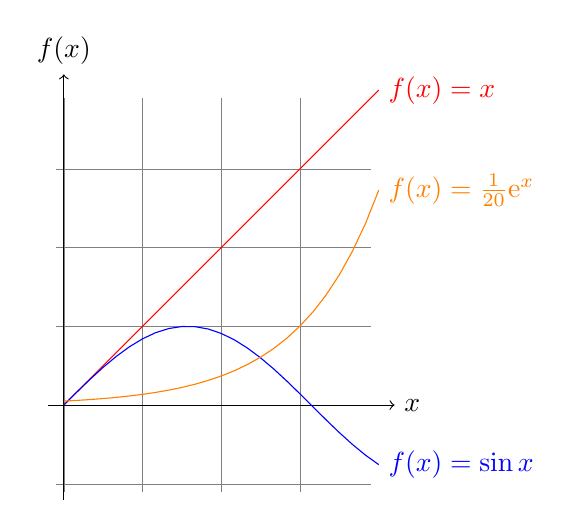
\begin{tikzpicture}[domain=0:4]
		  \draw[very thin,color=gray] (-0.1,-1.1) grid (3.9,3.9);
  		\draw[->] (-0.2,0) -- (4.2,0) node[right] {$x$};
		  \draw[->] (0,-1.2) -- (0,4.2) node[above] {$f(x)$};
		  \draw[color=red]    plot (\x,\x)             node[right] {$f(x) =x$};
  % \x r 表示弧度
		  \draw[color=blue]   plot (\x,{sin(\x r)})    node[right] {$f(x) = \sin x$};
		  \draw[color=orange] plot (\x,{0.05*exp(\x)}) node[right] {$f(x) = \frac{1}{20} \mathrm e^x$};
		\end{tikzpicture}
	\end{center}
\end{minipage}


\clearpage

\begin{minipage}<t>[htpb][80mm][t]{80mm}
	\begin{center}
		\vspace*{60mm}
    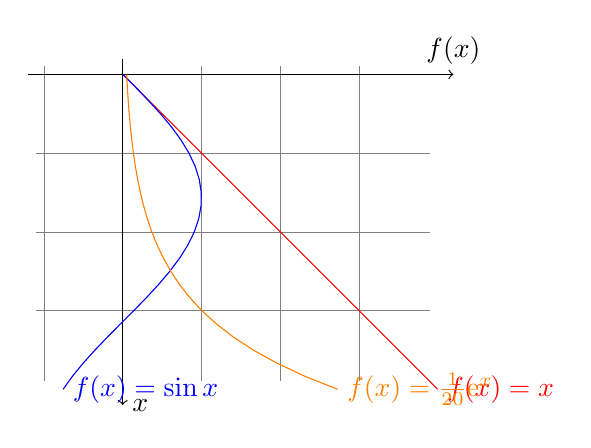
\begin{tikzpicture}[domain=0:4,scale=1,rotate=270]
		  \draw[very thin,color=gray] (-0.1,-1.1) grid (3.9,3.9);
  		\draw[->] (-0.2,0) -- (4.2,0) node[right] {$x$};
		  \draw[->] (0,-1.2) -- (0,4.2) node[above] {$f(x)$};
		  \draw[color=red]    plot (\x,\x)             node[right] {$f(x) =x$};
  % \x r 表示弧度
		  \draw[color=blue]   plot (\x,{sin(\x r)})    node[right] {$f(x) = \sin x$};
		  \draw[color=orange] plot (\x,{0.05*exp(\x)}) node[right] {$f(x) = \frac{1}{20} \mathrm e^x$};
		\end{tikzpicture}
	\end{center}
\end{minipage}

\chapter{公式測試}

\begin{minipage}<y>[htpb]{80mm}
		\vspace*{45mm}
	%\begin{center}
			{\normalsize With normalsize 10 pt in class (truely 9.13\,pt in real dimen):
				\[ \sampleEq \]\par}

			{\Large With Large 14 pt in class (truely 12.782\,pt in real dimen):
				\[ \sampleEq \]\par}

			{\footnotesize With footnotesize 8 pt in class (truely 7.304\,pt in real dimen):
				\[ \sampleEq \]\par}
	%\end{center}
\end{minipage}

\clearpage
\begin{minipage}<t>[htpb]{120mm}
		\vspace*{10mm}
	%\begin{center}
			{\normalsize 
				\[ \sampleEq \]\par}

			{\Large 
				\[ \sampleEq \]\par}

			{\footnotesize
				\[ \sampleEq \]\par}
	%\end{center}
\end{minipage}


\endinput